
\section{Geometría euclídea (del 25/01 al final)}

Llamamos geometría euclídea al espacio en el que podemos medir, cosa que hasta ahora no era posible.

Todo surge desde el módulo de un vector. Llamamos \concept[Módulo de un vector]{módulo de un vector} a la longitud que tiene. Dado $\vec{v}$, se define el módulo como $|\vec{v}|$.

\subsection{Producto, escalar, vectorial y mixto}

\paragraph{Introducción sobre el origen del producto escalar y vectorial}

Fuentes consultadas:
\begin{itemize}
  \item \href{http://www.suitcaseofdreams.net/Geometric_multiplication.htm}{Relación forma polar y binómica del producto complejo}
  \vspace{-0.4cm}
  \item \href{https://www2.clarku.edu/faculty/djoyce/complex/mult.html}{Interpretación geométrica del producto complejo}
  \vspace{-0.4cm}
  \item \href{https://www.quora.com/Who-invented-the-dot-product-and-cross-product}{Historia y aplicación de los cuaterniones los productos}
  \vspace{-0.4cm}
  \item \href{https://es.wikipedia.org/wiki/Cuaterni%C3%B3n}{ Extensión de los complejos al grupo de los quaterniones}
\end{itemize}

Dados 2 números complejos $z_1 = a_1+b_1i$, $z_2 = a_2+b_2i$. Expresando estos números complejos en forma polar tenemos: $z_1=r_{\alpha_1}$ y $z_2 = s_{\alpha_2}$.  

$z_1·z_2 = (a_1a_2 - b_1b_2) + (a_1b_2+a_2b_1)i = r·s_{\alpha_1+\alpha_2}$.

Tomando $z_1·\bar{z_2} = (a_1a_2 + b_1b_2) + (a_1b_2-a_2b_1)i = r·s_{\alpha_1-\alpha_2}
$

\subparagraph{Estudio de la parte real (producto escalar)}

En $Re(z_1·\bar{z_2}) = a_1a_2 + b_1b_2 = Re(r·s_{\alpha_1-\alpha_2})$

Para calcular $Re(r·s_{\alpha_1-\alpha_2}) = Re(r·s·\cos(\alpha_1-\alpha_2) + i·r·s·\sen(\alpha_1-\alpha_2)$, por lo que podemos completar:

$ a_1a_2 + b_1b_2 = |z_1||z_2|·\cos(\alpha_1-\alpha_2)$, y, siendo conscientes que $\alpha_1-\alpha_2$ es el ángulo que forman los 2 vectores, obtenemos la expresión del producto escalar de 2 vectores.


\subparagraph{Estudio de la parte imaginaria (producto vectorial)}

Al extender este razonamiento al grupo de los cuaterniones, tendríamos:

\newcommand{\quat}{\vec}

$Re(z_1\bar{z_2}) = Re\left((b_1\quat{i}+c_1\quat{j}+d_1\quat{k})·(-b_2\quat{i}-c_2\quat{j}-d_2\quat{k})\right) = (b_1b_2+c_1c_2+d_1d_2)$

Lo espectacular viene al considerar la parte "imaginaria" (aunque no tengamos claro cómo se define ese concepto en los cuaterniones):

$Im(z_1\bar{z_2}) = f(\quat{i},\quat{j},\quat{k})$, cuya expresión analítica es la del producto vectorial, ya que en grupo de los cuaterniones $\quat{i}\quat{j}=\quat{k}$ y todo eso.

\subsubsection{Producto escalar}

\begin{itemize}
  \item Definición.
  \item Base ortogonal y ortonormal.
  \item Expresión analítica.
  \item Cálculo del módulo (porque Pitágoras tridimensional no funciona).
  \item Base canónica.
  \item Interpretación geométrica (proyección).
\end{itemize}

\subsubsection{Producto vectorial}
\begin{itemize}
  \item Definición.
  \subitem Regla de la mano derecha
  \item Expresión analítica.
  \item Interpretación geométrica. 
\end{itemize}


\subsubsection{Producto mixto}

\begin{itemize}
  \item ¿Qué ocurre si en el producto vectorial meto un vector en lugar de $\vec{i},\vec{j},\vec{k}$?
  \item Definición.
  \item Expresión analítica.
  \item Interpretación geométrica. 
\end{itemize}

\subsubsection{Practicamos en general ejercicios del tema 9}

\subsection{Aplicación de los productos}

\subsubsection{Vector normal del plano}

\subsubsection{Vector director de la recta en implícitas}

\begin{figure}[hbtp]
\centering
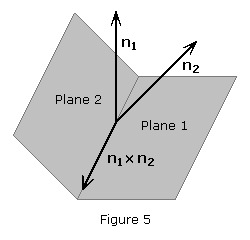
\includegraphics{img/directorrectaimplicitas.jpg}
\end{figure}

Dada una recta $r$ que pertenece a ambos planos, $\pi_1$ y $\pi_2$, $\vec{V_r}\perp n_{\pi_1} \wedge \vec{V_r}\perp n_{\pi_2}$. Por eso, para buscar un vector perpendicular a la vez a 2 vectores dados, el camino más corto es el producto vectorial.

$\vec{V_r} = n_{\pi_1}\times n_{\pi_2}$

\begin{problem}

Halla la recta perpendicular a $r:\frac{x-1}{2} = \frac{y+2}{3} = \frac{2z-2}{3}$ que pasa por el punto $P(1,-2,0)$.

\solution

La recta pedida es $t:\left\{\begin{array}{c}P\in t\\t\perp r\\\end{array}\right.$ 

Todas las rectas perpendiculares a una recta forman un plano. Llamamos $\pi$ a ese plano. Así, $ t \in \pi, \text{ con } \pi:\left\{\begin{array}{c}P\in\pi\\\pi\perp r\end{array}\right.$. Así, $t$ será la recta determinada por $A = t\cap\pi, P(1,-2,0)$

$\pi\perp r\implies n_{\pi} || \vec{V_r}$. Tomamos $n_{\pi}  = \left(2,3,\rfrac{3}{2}\right)$

Como $P\in\pi\implies 2P_1 + 3P_2 +\rfrac{3}{2}P_3 + D = 0 \dimplies 2-6+D = 0 \dimplies D=4$

Así, $\pi: 2x+3y+\rfrac{3}{2}z + 4 = 0$

2) Buscamos $A=\pi\cap r$. Tendremos $t:\{A,P\}$


\[
  \left\{\begin{array}{c}
    2x+3y+\rfrac{3}{2}z + 4 = 0\\
    x = 1 + 2\lambda\\
    y = -2 + 3\lambda\\
    z = 1 + \rfrac{3}{2}\lambda\end{array}\right\} \implies 2+4\lambda - 6 + 9\lambda + \rfrac{3}{2} + \rfrac{9}{4}\lambda + 4 = 0 \dimplies 
\]
\[
  \frac{3}{2}+\left(13+\rfrac{9}{4}\right)\lambda = 0 \dimplies \lambda = \frac{\rfrac{61}{4}}{\rfrac{3}{2}} = \frac{61}{6}
\]

Sustituimos $\lambda$ en la ecuación de la recta para obtener $A$:
$\left\{\begin{array}{c}
    x = 1 + 2\rfrac{61}{6} = \frac{64}{3}\\
    y = -2 + 3\rfrac{61}{6} = \frac{57}{2}\\
    z = 1 + \rfrac{3}{2}\rfrac{61}{6} = \frac{57}{4}
\end{array}\right\}$


\[A = \pi\cap r = \left(\frac{64}{3},\frac{57}{2},\frac{57}{4}\right)\]

3) Buscamos la recta $r$ que pasa por los puntos $A$ y $P$. 

$\vec{AP} = \left(\frac{64}{3}-1,\frac{57}{2}+2,\frac{57}{4}\right) =  \left(\frac{61}{3},\frac{61}{2},\frac{57}{4}\right)$

\[r : \{A,\vec{V_r}\} = \left\{\begin{array}{c}
    x = \rfrac{64}{3} + 2\lambda\\
    y = \rfrac{57}{2} + 3\lambda\\
    z = \rfrac{57}{4} + \rfrac{3}{2}\lambda
\end{array}\right\}\]

\end{problem}

127,128.

\begin{problem}[Junio 2019]

Dados los puntos $A(1,1,1), B(1,3,-3)$ y $C(-3,-1,1)$, se pide:
\ppart Determinar la ecuación del plano que contiene a los 3 puntos.
\ppart Obtener un punto $D$ (distinto a los anteriores) tal que los vectores $\vec{AB}$, $\vec{AC}$,$\vec{AD}$ sean linealmente dependientes.
\ppart Encontrar un punto $P$ del eje $OX$, de modo que el volumen del tetraedro de vértices $A$,$B$,$C$,$P$ sea igual a 1.

\solution

\spart 

Tomamos $\vec{AB} = (0,2,-4)$, $\vec{AC} = (-4,-2,0)$ como vectores directores del plano y calculamos su ecuación implícita:

\[
\pi: \left|\begin{array}{ccc}
x - 1 & 0 & -4\\
y - 1 & 2 & -2\\
z - 1 & -4& 0
\end{array}\right| = 0 \dimplies 16y-16 + 8z-8-8x+8 = 0\]
\[\dimplies -8x + 16y + 8z -16 = 0 \dimplies -x+2y+z-2=0
\]

\spart Basta con tomar $D\in\pi$. Por ejemplo: $D(0,1,0)\in\pi$.

Comprobamos que $\vec{AB},\vec{AC},\vec{AD}$ son linealmente dependientes calculando el determinante de la matriz que forman.

$\vec{AD} = (1,0,1)$

\[
|\vec{AB}\quad\vec{AC}\quad\vec{AD}| = 
\left|\begin{array}{ccc}
1 & 0 & -4\\
0 & 2 & -2\\
1 & -4& 0
\end{array}\right| = 0
\]

\spart 

(Ojo que aquí no se puede simplificar, aunque antes sí hubiéramos podido)

El volumen del tetraedro será $\rfrac{1}{6}$ del voluen del paralelepípedo:

\[
||\vec{AB}\quad\vec{AC}\quad\vec{AD}|| = 
\left|\left|\begin{array}{ccc}
1 & 0 & -4\\
1 & 2 & -2\\
a-1 & -4& 0
\end{array}\right|\right| = 2·2·\left|\left|\begin{array}{ccc}
1 & 0 & 2\\
1 & 1 & 1\\
z-1 & -2& 0
\end{array}\right|\right| = {6} 
\]
\[
 \left|\left|\begin{array}{ccc}
1 & 0 & 2\\
1 & 1 & 1\\
a-1 & -2& 0
\end{array}\right|\right| = \frac{3}{2}  \dimplies
|-4 -2a-2+2| = \frac{3}{2}\dimplies |-4-2a| = \rfrac{3}{2} \implies\]
\[
\left\{\begin{array}{c}
-4-2a_1 = \rfrac{3}{2} \dimplies a_1 = \frac{-11}{4} \to P_1\left(\rfrac{-11}{4},0,0\right)\\
4+2a_2 = \rfrac{3}{2} \dimplies a_2 = \frac{-5}{4} \to P_2\left(\rfrac{-5}{4},0,0\right)
\end{array}\right.
\]

\end{problem}


\subsection{Perpendicular común}


\subsection{Proyecciones y simetrías}

\subsubsection{Proyección}

\subsubsection{Simetría de un punto respecto de otro punto}

Tirao.

\subsubsection{Simetría de un punto respecto de una recta}

Plano perpendicular a la recta que contenga al punto, intersección con la recta.

\subsubsection{Simetría de un punto respecto de un plano}

Recta perpendicular al plano, que pasa por el punto.

\newpage
\subsection{Ángulos}
\subsubsection{Ángulo formado por dos rectas: secantes, se cruzan y paralelas/coincidentes}
\subsubsection{Ángulo formado por dos planos}
\subsubsection{Ángulo formado por recta y plano}

\subsection{Distancias}
\subsubsection{Entre 2 puntos}
\subsubsection{Plano mediador}
\subsubsection{Entre punto y plano}
\subsubsection{Planos bisectores}
\subsubsection{Entre 2 planos}
\subsubsection{Entre recta y plano}
\subsubsection{Entre punto y recta}
\subsubsection{Entre 2 rectas paralelas}
\subsubsection{Entre 2 rectas no paralelas}

\subsubsection{Volumen del paralelepípedo}
